\subsection{基礎量と記法}

机の上で小さな台車がばねとダンパにつながれており、モータの力で原点へ戻したいとする。センサからは、位置、速度、モータが出せる力の上限が得られる。測定結果を単に
\begin{equation}
  0.08,\qquad -0.12,\qquad 1.5
\end{equation}
と並べただけでは、台車が原点から $8\,\mathrm{cm}$ 離れているのか、$0.08\,\mathrm{m}$ 離れているのか、速度が $-0.12\,\mathrm{m/s}$ なのか、入力上限が $1.5\,\mathrm{N}$ なのかを判定できない。制御器は数値を計算するが、モデル化の段階では、その数値が何を測ったものかを失うと式の意味が崩れる。

たとえば、時刻 $t$ の位置が $q(t)=0.08\,\mathrm{m}$、速度が $\dot{q}(t)=-0.12\,\mathrm{m/s}$ であるなら、$0.10\,\mathrm{s}$ 後に速度だけで進む距離は
\begin{equation}
  \dot{q}(t)\Delta t
  =
  -0.12\,\frac{\mathrm{m}}{\mathrm{s}}\cdot0.10\,\mathrm{s}
  =
  -0.012\,\mathrm{m}
\end{equation}
である。したがって、短い時間だけ速度がほぼ一定だとみなせば、次の位置は
\begin{equation}
  q(t+\Delta t)\simeq q(t)+\dot{q}(t)\Delta t
  =0.08\,\mathrm{m}-0.012\,\mathrm{m}
  =0.068\,\mathrm{m}
\end{equation}
と計算できる。一方、$q(t)+\dot{q}(t)$ のように位置と速度をそのまま足しても、長さと長さ毎秒の和になり、物理量として解釈できない。この段階で必要になる最初の言葉が、量と単位である。

\begin{definition}[量と単位]
数値と単位を合わせたものを量という。たとえば $3\,\mathrm{s}$ は時間、$5\,\mathrm{m}$ は長さ、$12\,\mathrm{V}$ は電圧を表す量である。
\end{definition}

量として書けば、数値の意味は測定の基準と結び付く。$10$ という数だけでは対象を決められないが、$10\,\mathrm{m}$ は長さ、$10\,\mathrm{s}$ は時間、$10\,\mathrm{rad/s}$ は角速度である。制御器の式は最終的にはプログラムや回路へ実装されるが、実装前の紙の上でも、単位を追うだけで多くの誤りを見つけられる。

単位を変えても、同じ種類の量であることは変わらない。$0.08\,\mathrm{m}$ と $8\,\mathrm{cm}$ は数値と単位の組としては異なるが、どちらも長さである。反対に、$0.08\,\mathrm{m}$ と $0.08\,\mathrm{s}$ は数値が同じでも量の種類が異なる。そこで、単位の選び方よりも粗く、量の種類を表す分類を導入する。

\begin{definition}[次元]
量がどの種類の物理量であるかを表す分類を次元という。長さの次元を $L$、時間の次元を $T$、質量の次元を $M$ と書くと、速度の次元は $LT^{-1}$、加速度の次元は $LT^{-2}$、力の次元は $MLT^{-2}$ である。
\end{definition}

単位は m、s、kg、V、A、rad/s のような具体的な測り方であり、次元はその背後にある量の種類である。同じ長さでも m、cm、mm は単位が違うだけで次元は同じ $L$ である。角度 rad は、弧長を半径で割った比なので次元を持たない。ただし、回転量であることを見失わないように単位記号として rad を残す。

等式を立てるときは、単位の表記だけでなく次元もそろっていなければならない。台車の位置予測で $q+\dot{q}\Delta t$ が意味を持ったのは、$\dot{q}\Delta t$ の次元が
\begin{equation}
  LT^{-1}\cdot T=L
\end{equation}
となり、位置 $q$ と同じ長さに戻ったためである。このように、式の両側と足し合わせる各項の種類がそろっているかを調べる条件を次元整合性という。

\begin{definition}[次元整合性]
物理量を含む等式で、左辺と右辺の次元が一致していることを次元整合性という。和や差を取る量は、同じ次元でなければならない。
\end{definition}

台車をもう少し詳しくモデル化すると、質量 $m$、粘性係数 $c$、ばね定数 $k$、位置 $q$、入力力 $u$ を用いて、質量ばねダンパ系
\begin{equation}
  m\ddot{q}+c\dot{q}+kq=u
\end{equation}
を得る。ここで $\ddot{q}$ は位置を時間で二回変化させた量であり、加速度である。位置の単位を m、時間の単位を s、力の単位を N とすると、
\begin{align}
  [m\ddot{q}]&=\mathrm{kg}\cdot\frac{\mathrm{m}}{\mathrm{s}^2}
    =\mathrm{N},\\
  [c\dot{q}]&=\frac{\mathrm{N\,s}}{\mathrm{m}}\cdot
    \frac{\mathrm{m}}{\mathrm{s}}
    =\mathrm{N},\\
  [kq]&=\frac{\mathrm{N}}{\mathrm{m}}\cdot\mathrm{m}
    =\mathrm{N}.
\end{align}
三つの項はいずれも力の単位を持つので、右辺の入力力 $u$ と足し合わせられる。もし $c$ の単位を誤って $\mathrm{N/m}$ と置けば、$c\dot{q}$ の単位は $\mathrm{N/s}$ になり、この式は物理量の等式として成立しない。

\begin{example}[RC 回路の時定数の次元確認]
電気回路でも同じ検査を使う。抵抗 $R$ と静電容量 $C$ からなる RC 回路では、入力電圧を急に変えてもコンデンサ電圧はすぐには変わらず、代表的な変化時間として時定数 $\tau=RC$ が現れる。抵抗の単位は $\Omega=\mathrm{V/A}$、静電容量の単位は $\mathrm{F}=\mathrm{C/V}$ であり、電荷の単位 C は $\mathrm{A\,s}$ である。したがって
\begin{align}
  [RC]
  &=\frac{\mathrm{V}}{\mathrm{A}}\cdot
    \frac{\mathrm{C}}{\mathrm{V}}\\
  &=\frac{\mathrm{C}}{\mathrm{A}}\\
  &=\frac{\mathrm{A\,s}}{\mathrm{A}}\\
  &=\mathrm{s}.
\end{align}
指数関数 $e^{-t/(RC)}$ の指数は無次元でなければならないので、$RC$ が時間の単位を持つことは式の形とも一致している。
\end{example}

単位と次元は、式が物理として成立するかを確認するために必要である。さらに、異なる大きさの実験や異なる単位系の結果を同じ図で比較したいときは、量を基準量で割って無次元の比へ直す。温度偏差 $\theta(t)$ が基準偏差 $\theta_0$ と同じ単位を持つなら
\begin{equation}
  x(t)=\frac{\theta(t)}{\theta_0}
\end{equation}
は無次元である。時刻も時定数 $\tau$ で割って
\begin{equation}
  \xi=\frac{t}{\tau}
\end{equation}
とすれば、一次遅れの式
\begin{equation}
  \tau\dot{\theta}+\theta=0
\end{equation}
は
\begin{equation}
  \frac{\dd x}{\dd \xi}+x=0
\end{equation}
と書ける。このように基準量で割って無次元量を作ることを無次元化という。無次元化は、単位を m から cm へ替える操作ではなく、基準値に対して何倍かを表す操作である。この区別を明確にするため、次に単位変換と正規化を同じ一次遅れのデータで比較する。

\subsubsection{単位変換と正規化の比較}

単位変換と正規化は、どちらも同じ物理量の数値表現を変える操作であるが、目的が異なる。単位変換では、対象とする物理量そのものは保ったまま、測る単位だけを変える。たとえば $30\,\mathrm{s}$ は $0.5\,\mathrm{min}$ と同じ時間であり、温度偏差 $10\,\mathrm{K}$ は華氏温度差では $18\,^\circ\mathrm{F}$ の差である。数値は単位の選び方で変わるが、次元を持つ量であることは変わらない。

一方、正規化では、同じ次元を持つ基準量で割る。熱系の温度偏差を
\begin{equation}
  \theta(t)=T(t)-T_{\mathrm{amb}}
\end{equation}
とし、周囲温度 $T_{\mathrm{amb}}$ が一定、初期偏差が $\theta_0=20\,\mathrm{K}$、時定数が $\tau=60\,\mathrm{s}$ であるケース A の一次遅れ
\begin{equation}
  \theta(t)=\theta_0 e^{-t/\tau}
\end{equation}
を仮定する。ここで $\theta$ は温度差なので、絶対温度の摂氏・華氏換算ではなく、差の単位変換だけを扱う。華氏温度差を $\theta_F$ と書けば、
\begin{equation}
  \theta_F=\frac{9}{5}\theta
\end{equation}
である。正規化時刻と正規化偏差を
\begin{equation}
  \xi=\frac{t}{\tau},\qquad
  x=\frac{\theta}{\theta_0}
\end{equation}
と定めると、表のように、同じ測定点を単位つきの量と無次元比の両方で表せる。

\begin{center}
\small
\begin{tabular}{c|c|c|c|c}
$t$ [s] & $\theta$ [K] & $\theta_F$ [$^\circ\mathrm{F}$ の差] & $\xi=t/\tau$ & $x=\theta/\theta_0$ \\
\hline
$0$ & $20.0$ & $36.0$ & $0.0$ & $1.00$ \\
$30$ & $12.1$ & $21.8$ & $0.5$ & $0.61$ \\
$60$ & $7.4$ & $13.2$ & $1.0$ & $0.37$ \\
$120$ & $2.7$ & $4.9$ & $2.0$ & $0.14$
\end{tabular}
\end{center}

この表では、$12.1\,\mathrm{K}$ と $21.8\,^\circ\mathrm{F}$ の差は同じ温度偏差である。したがって、単位変換は物理量を変えず、数値と単位記号の組を変える操作である。これに対して、$x=0.61$ は温度差そのものではなく、初期偏差の $61\,\%$ に相当するという無次元の比である。$\xi=0.5$ も $30\,\mathrm{s}$ という時間ではなく、時定数の半分だけ経過したことを表す。

無次元化により、単位系に依存しない本質的なパラメータが明確になる。ケース A を $\theta_0=20\,\mathrm{K}$、$\tau=60\,\mathrm{s}$ とし、別の実験であるケース B を $\theta_0=10\,\mathrm{K}$、$\tau=120\,\mathrm{s}$ とする。どちらも同じ一次遅れであれば、正規化した応答は
\begin{equation}
  x(\xi)=e^{-\xi}
\end{equation}
に重なる。この対応は、同じ正規化時刻で二つの実験を並べると確認できる。

\begin{center}
\small
\begin{tabular}{c|cc|cc|c}
& \multicolumn{2}{c|}{ケース A} & \multicolumn{2}{c|}{ケース B} & \\
$\xi$ & $t$ [s] & $\theta$ [K] & $t$ [s] & $\theta$ [K] & $x=e^{-\xi}$ \\
\hline
$0.5$ & $30$ & $12.1$ & $60$ & $6.1$ & $0.61$ \\
$1.0$ & $60$ & $7.4$ & $120$ & $3.7$ & $0.37$
\end{tabular}
\end{center}

\begin{figure}[tb]
\centering
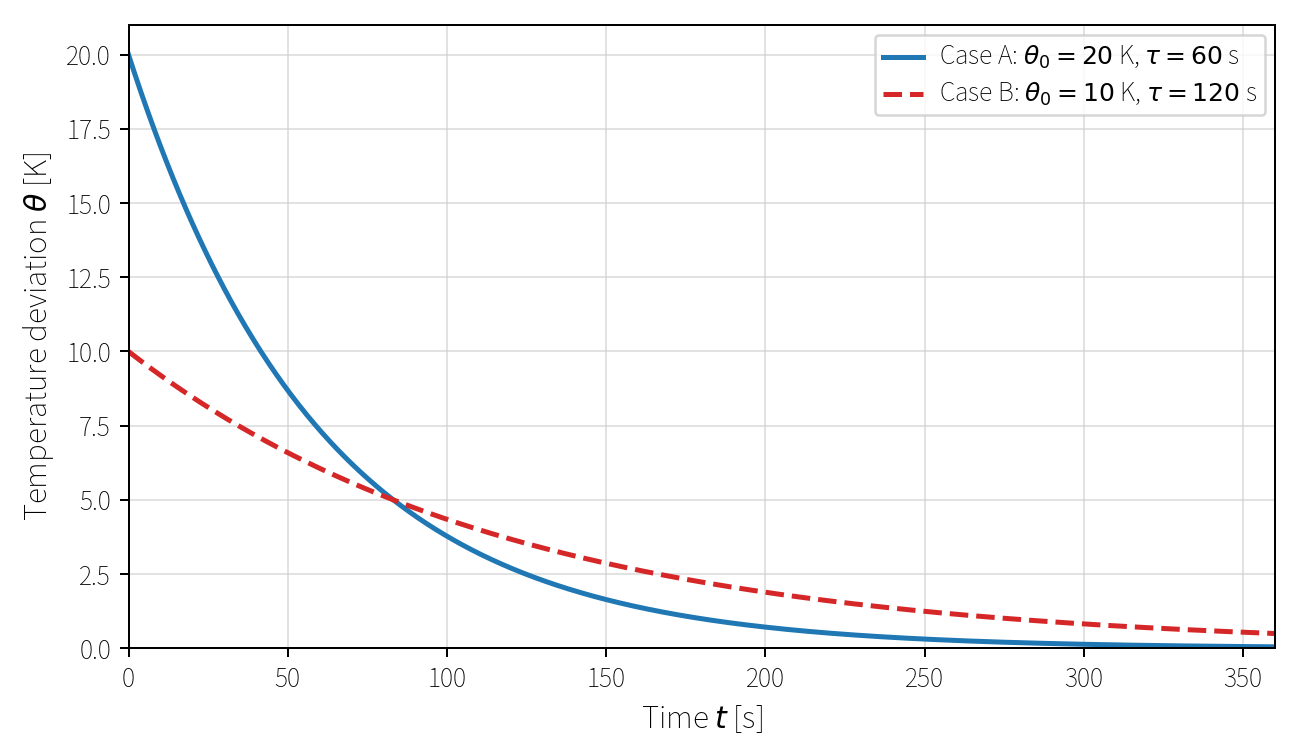
\includegraphics[width=0.86\linewidth,bb=0 0 1296 756]{figures/unit_response_dimensional.png}
\caption{ケース A $(\theta_0=20\,\mathrm{K},\,\tau=60\,\mathrm{s})$ とケース B $(\theta_0=10\,\mathrm{K},\,\tau=120\,\mathrm{s})$ を、次元つきの時間 $t$ と温度偏差 $\theta$ で描いた一次遅れ応答。初期偏差と時定数が異なるため、曲線の高さと減衰速度が異なる。}
\label{fig:unit-normalization-dimensional}
\end{figure}

\begin{figure}[tb]
\centering
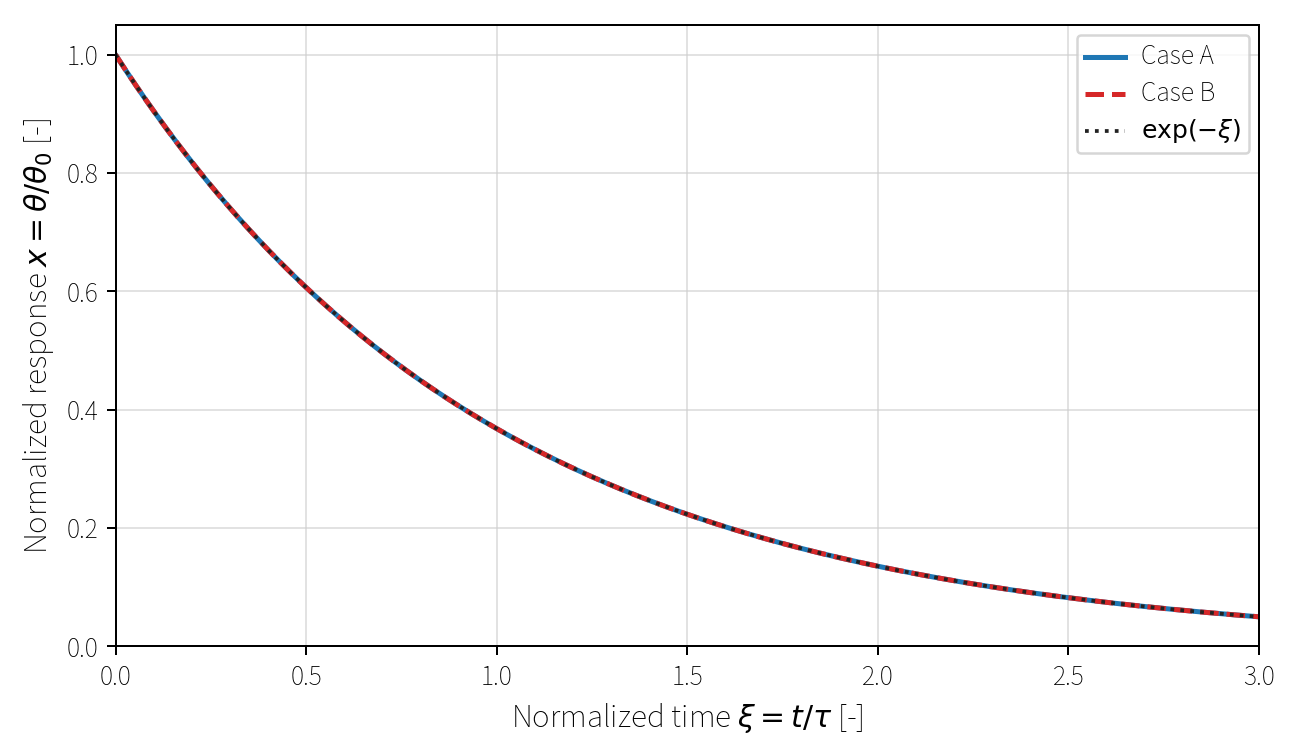
\includegraphics[width=0.86\linewidth,bb=0 0 1296 756]{figures/unit_response_normalized.png}
\caption{$\xi=t/\tau$ と $x=\theta/\theta_0$ で正規化した一次遅れ応答。二つの実験が $x=e^{-\xi}$ に重なるため、単位や実験スケールを越えて同じ減衰過程として比較できる。}
\label{fig:unit-normalization-example}
\end{figure}

図\ref{fig:unit-normalization-dimensional} と図\ref{fig:unit-normalization-example} は、上の比較表を連続曲線として表したものである。次元つきの図では実験ごとの初期偏差と時定数がそのまま曲線を変えるが、正規化した図では表の最後の列と同じ無次元応答へ整理される。この比較では、ケース B の時定数がケース A の 2 倍であるため、同じ $\xi$ に到達する実時間 $t$ は 2 倍になる。また、ケース B の初期偏差はケース A の半分なので、同じ $\xi$ における温度偏差 $\theta$ も半分になる。それでも最後の列の $x$ は一致する。したがって、異なる実験の温度値や時間値を直接比較する代わりに、何時定数分だけ経過したか、初期偏差の何割まで減ったかを比較できる。制御器の調整でも、図\ref{fig:unit-normalization-example} と同じように状態を許容偏差で割り、時間を代表時定数で割っておくと、ゲインや評価関数の重みが単位の選び方に過度に依存しにくくなる。

\begin{practice}[単位変換と正規化の確認]
上の比較表と同じ二つのケースで $\xi=1.5$ とする。各ケースの $t$、$\theta(t)$、華氏温度差、$x$ を求めよ。単位つきの $t$ と $\theta$ は異なるが、無次元量 $x$ は一致することを確認せよ。
\end{practice}

\subsection{変数と関数}

制御では、対象を動かす前に、望む値と実際の値を時間順に記録する。たとえば温度を $30\,^\circ\mathrm{C}$ に保ちたい実験で、測定値と入力を次のように並べる。
\begin{center}
\begin{tabular}{c|rrrr}
時刻 $t$ [s] & 0 & 1 & 2 & 3\\
\hline
目標値 $r$ [$^\circ\mathrm{C}$] & 30.0 & 30.0 & 30.0 & 30.0\\
測定出力 $y$ [$^\circ\mathrm{C}$] & 24.0 & 26.5 & 28.1 & 29.0\\
入力 $u$ [\%] & 80 & 55 & 35 & 22\\
偏差 $e=r-y$ [$^\circ\mathrm{C}$] & 6.0 & 3.5 & 1.9 & 1.0
\end{tabular}
\end{center}
この表では、どの数が時刻で、どの数が目標値、測定出力、入力、偏差であるかを区別しなければ、制御計算を再現できない。さらに、測定出力や入力は時刻とともに変わるため、一つの固定値ではなく、時刻に応じて変化する量として扱う必要がある。この必要から、値が変わる量に名前を与え、その名前と時刻などの条件との対応を記述する。

\begin{definition}[変数]
値が状況によって変わる記号を変数という。時刻を $t$、位置を $q$、速度を $v$、入力を $u$ と書くとき、それらは変数である。
\end{definition}

\begin{definition}[関数]
ある値を入れると別の値が決まる対応を関数という。時刻 $t$ を入れると位置 $q(t)$ が決まるとき、$q$ は時刻の関数である。
\end{definition}

上の測定表では、測定出力を $y(t)$、入力を $u(t)$、偏差を $e(t)$ と書けば、時刻を指定したときの値を明確に表せる。関数 $q(t)$ は、表、グラフ、または式で表される。たとえば一定速度 $v_0$ で動く物体の位置は
\begin{equation}
  q(t)=q(0)+v_0t
\end{equation}
と書ける。ここで $q(0)$ は時刻 0 の位置である。$t=2$ を代入すれば
\begin{equation}
  q(2)=q(0)+2v_0
\end{equation}
となる。関数は、入力値に対して出力値を一意に対応させる写像である。

関数を評価するときは、式だけでなくグラフも使う。横軸に入力、縦軸に出力を取り、入力を少し変えたときに出力がどの向きへどれだけ変わるかを確認する。制御では、横軸を時刻 $t$、縦軸を出力 $y(t)$ とした応答グラフ、横軸を入力 $u$、縦軸を静的な出力 $y$ とした特性グラフ、横軸を周波数、縦軸をゲインまたは位相とした周波数応答グラフを使う。

\begin{definition}[比例]
一方の量 $x$ が $a$ 倍になると、もう一方の量 $y$ も同じく $a$ 倍になる関係を比例という。定数 $K$ を用いて
\begin{equation}
  y=Kx
\end{equation}
と書ける。
\end{definition}

比例定数 $K$ は、入力 1 単位あたりの出力変化である。単位は $y$ の単位を $x$ の単位で割ったものになる。ばねの力を
\begin{equation}
  F=kq
\end{equation}
と書くなら、$F$ の単位は N、$q$ の単位は m なので、ばね定数 $k$ の単位は $\mathrm{N/m}$ である。電気回路で抵抗に流れる電流を
\begin{equation}
  i=\frac{1}{R}v
\end{equation}
と書くなら、電圧 $v$ と電流 $i$ は比例し、比例定数 $1/R$ はコンダクタンスである。

\begin{definition}[反比例]
一方の量 $x$ が大きくなると、もう一方の量 $y$ がその逆数に比例して小さくなる関係を反比例という。定数 $K$ を用いて
\begin{equation}
  y=\frac{K}{x},\qquad x\ne0
\end{equation}
と書ける。
\end{definition}

反比例は、一定の積を保つ関係として現れる。一定距離 $d$ を速度 $v$ で移動する時間 $T$ は
\begin{equation}
  T=\frac{d}{v}
\end{equation}
である。距離 $d$ を固定すると、速度を 2 倍にすれば時間は半分になる。制御対象の設計では、帯域を上げると遅れ時間に対する余裕が小さくなる、サンプリング周期を短くすると 1 秒あたりの計算回数が増える、といった場面で同じ関係を使う。

\begin{definition}[一次関数とアフィン関数]
定数 $a,b$ を用いて
\begin{equation}
  y=ax+b
\end{equation}
と書ける関数を一次関数という。線形代数では、$b=0$ の場合を線形、$b\ne0$ を許す場合をアフィンと呼ぶことが多い。
\end{definition}

一次関数のグラフは直線である。$a$ は傾きであり、$x$ を $\Delta x$ だけ増やしたとき出力が
\begin{equation}
  \Delta y=a\Delta x
\end{equation}
だけ変わることを表す。$b$ は切片であり、$x=0$ のときの出力である。温度センサの校正式
\begin{equation}
  V=S\theta+V_0
\end{equation}
では、$\theta$ が温度、$V$ が電圧、$S$ が感度、$V_0$ がオフセットである。制御では、平衡点まわりの小さな変化だけを見ると、多くの非線形関数が一次関数として近似される。

\begin{definition}[二次関数]
定数 $a,b,c$ を用いて
\begin{equation}
  y=ax^2+bx+c,\qquad a\ne0
\end{equation}
と書ける関数を二次関数という。
\end{definition}

二次関数のグラフは放物線である。$a>0$ なら上に開き、$a<0$ なら下に開く。平方完成により
\begin{align}
  ax^2+bx+c
  &=a\left(x^2+\frac{b}{a}x\right)+c\\
  &=a\left\{\left(x+\frac{b}{2a}\right)^2
    -\left(\frac{b}{2a}\right)^2\right\}+c\\
  &=a\left(x+\frac{b}{2a}\right)^2
    +c-\frac{b^2}{4a}
\end{align}
となる。したがって頂点は
\begin{equation}
  x=-\frac{b}{2a}
\end{equation}
にある。二次関数は、エネルギー、二乗誤差、LQR や MPC の評価関数を扱うための基本形である。たとえば目標値 $r$ に対する偏差 $e=y-r$ を小さくしたいとき、評価
\begin{equation}
  J=e^2
\end{equation}
は $e=0$ で最小になり、正負どちらの偏差も同じように罰する。入力を大きくしたくないときは $u^2$ を加え、後で
\begin{equation}
  J=e^2+\rho u^2,\qquad \rho>0
\end{equation}
のような形へ進む。

\subsection{三角関数、指数関数、対数関数}

制御対象の記録には、直線や放物線だけでは表しにくい変化が繰り返し現れる。振子や質量ばねダンパ系の変位は、目標値の上下に振れながら振動する。温度差や RC 回路のコンデンサ電圧は、一定時間ごとに同じ割合で小さくなるような減衰を示す。正弦波の入力を加えて実験すると、入力振幅に対する出力振幅の比や位相のずれを周波数ごとに記録することになる。

このような振動、減衰、ゲイン比を同じ数式表現で扱うために、三角関数、指数関数、対数関数を用いる。三角関数は角度と周期運動を、指数関数は一定割合で増減する量を、対数関数は比や桁の違いを表す。振子の小振幅運動、質量ばねダンパ系の変位、回転角、温度差、RC 回路のコンデンサ電圧は、以下で導入する関数形で記述される。

\subsubsection{ラジアンと単位円}

角度を度で表すと、直角は $90^\circ$、一周は $360^\circ$ である。解析式では、弧長と半径の比により定まるラジアンを用いる。

\begin{definition}[ラジアン]
半径 $r$ の円で、中心角 $\theta$ が切り取る弧の長さを $s$ とする。このとき
\begin{equation}
  \theta=\frac{s}{r}
\end{equation}
で定まる角度の単位を rad と書き、ラジアンという。
\end{definition}

弧の長さ $s$ と半径 $r$ はどちらも m なので、比 $s/r$ は無次元である。ただし、角度を表す量であることを明示するために $\mathrm{rad}$ を添える。半径 $r$ の円を一周すると弧の長さは $2\pi r$ であるから、一周の角度は
\begin{equation}
  \theta=\frac{2\pi r}{r}=2\pi\,\mathrm{rad}
\end{equation}
である。したがって
\begin{equation}
  180^\circ=\pi\,\mathrm{rad},
  \qquad
  1^\circ=\frac{\pi}{180}\,\mathrm{rad}
\end{equation}
となる。

\begin{definition}[単位円による三角関数]
半径 1 の円を単位円という。原点から角度 $\theta$ だけ回した点の座標を
\begin{equation}
  (x,y)=(\cos\theta,\sin\theta)
\end{equation}
と定める。この $\cos\theta$ と $\sin\theta$ をそれぞれ余弦、正弦という。
\end{definition}

単位円上の点の座標は常に
\begin{equation}
  x^2+y^2=1
\end{equation}
を満たす。したがって
\begin{equation}
  \cos^2\theta+\sin^2\theta=1
\end{equation}
である。この恒等式は、正弦波の振幅、回転行列の長さ保存性、位相差を含む二乗和の評価に用いられる。

\begin{definition}[正弦波]
振幅 $A$、角周波数 $\omega$、初期位相 $\phi$ を用いて
\begin{equation}
  q(t)=q_0+A\sin(\omega t+\phi)
\end{equation}
と書ける信号を正弦波という。$q_0$ は中心値である。
\end{definition}

ここで $q(t)$ が位置なら $q_0$ と $A$ の単位は m、$q(t)$ が電圧なら V である。一方、$\sin$ の中身 $\omega t+\phi$ は角度なので無次元でなければならない。時刻 $t$ の単位が s であるから、$\omega$ の単位は $\mathrm{rad/s}$ である。

正弦波が同じ値を繰り返す最小の正の時間を周期 $T$ と呼ぶ。$\sin$ は角度が $2\pi$ 増えると同じ値を取るので、周期は
\begin{align}
  \omega(t+T)+\phi&=\omega t+\phi+2\pi,\\
  \omega T&=2\pi,\\
  T&=\frac{2\pi}{\omega}
\end{align}
である。1 秒あたりに何周期あるかを周波数 $f$ と呼ぶと、$f=1/T$ だから
\begin{equation}
  \omega=2\pi f
\end{equation}
である。$f$ の単位は Hz、すなわち $1/\mathrm{s}$ である。

\begin{example}[質量ばねの変位]
摩擦を無視した質量ばね系では、平衡位置からの変位が近似的に
\begin{equation}
  q(t)=A\sin(\omega t+\phi)
\end{equation}
と書ける。ここで $A$ は最大変位、$\omega$ は角周波数、$\phi$ は初期位相である。同じ $A$ に対して $\omega$ が大きいほど周期 $T=2\pi/\omega$ は短い。二次遅れ系では $\omega$ が振動成分の角周波数を表し、周波数応答では入力正弦波の角周波数を表す。
\end{example}

\subsubsection{指数関数と時定数}

指数関数は、単位時間あたりの相対変化率が一定である変化を表す。目標値からの偏差、温度差、電圧、速度誤差の一次近似では指数関数が現れる。

\begin{definition}[指数関数]
正の定数 $a$ に対して、入力 $x$ を与えると $a^x$ を返す関数を指数関数という。特に、自然対数の底
\begin{equation}
  e\simeq 2.71828
\end{equation}
を底にした $e^x$ は、連続時間の微分方程式の解に現れる。
\end{definition}

指数関数の指数 $x$ は無次元でなければならない。したがって、時刻を指数に入れるときは
\begin{equation}
  e^{-t/\tau}
\end{equation}
のように、時間 $t$ を同じ単位の定数 $\tau$ で割る。ここで $\tau$ の単位は s である。

\begin{definition}[時定数]
量 $x(t)$ が
\begin{equation}
  x(t)=x(0)e^{-t/\tau},\qquad \tau>0
\end{equation}
で変化するとき、$\tau$ を時定数という。
\end{definition}

時刻 $t=\tau$ を代入すると
\begin{equation}
  x(\tau)=x(0)e^{-1}\simeq0.368x(0)
\end{equation}
である。したがって、時定数は初期値に対する比が $e^{-1}\simeq0.368$ となる時間である。$2\tau$、$3\tau$、$5\tau$ では
\begin{align}
  x(2\tau)&=x(0)e^{-2}\simeq0.135x(0),\\
  x(3\tau)&=x(0)e^{-3}\simeq0.050x(0),\\
  x(5\tau)&=x(0)e^{-5}\simeq0.0067x(0)
\end{align}
となる。したがって、一次遅れ系の偏差は数時定数の経過後に初期偏差の小さい割合まで減衰する。

\begin{example}[RC 回路の電圧]
抵抗 $R$ とコンデンサ $C$ だけで放電する RC 回路では、コンデンサ電圧 $v_C(t)$ が
\begin{equation}
  v_C(t)=v_C(0)e^{-t/(RC)}
\end{equation}
で減る。したがって時定数は
\begin{equation}
  \tau=RC
\end{equation}
である。抵抗の単位 $\Omega$ と静電容量の単位 F の積は s になるので、$t/(RC)$ は無次元である。$R=10\,\mathrm{k}\Omega$、$C=100\,\mu\mathrm{F}$ なら
\begin{equation}
  \tau=10\times10^3\cdot100\times10^{-6}=1\,\mathrm{s}
\end{equation}
であり、約 3 秒後に初期電圧の $5\%$ 程度まで下がる。
\end{example}

指数関数は減衰だけでなく増大も表す。
\begin{equation}
  x(t)=x(0)e^{at},\qquad a>0
\end{equation}
なら、$a$ の単位は $1/\mathrm{s}$ であり、$x(t)$ は時間とともに増加する。不安定な閉ループの偏差や正帰還を含む系の応答では、この形の指数増大が現れる。

\subsubsection{対数と dB}

対数は、指数関数の逆関数であり、倍率を加法的な量へ変換する。ゲインの積を和として扱う場合、および広い範囲の振幅比を同一の尺度で表示する場合に用いる。

\begin{definition}[対数]
底 $a$ が $a>0$、$a\ne1$ を満たすとする。$a^x=b$ を満たす $x$ を
\begin{equation}
  x=\log_a b
\end{equation}
と書き、底 $a$ の対数という。対数の中身 $b$ は正の無次元量でなければならない。
\end{definition}

自然対数は底が $e$ の対数であり、単に $\log b$ と書く。常用対数は底が 10 の対数であり、$\log_{10}b$ と書く。指数減衰の時刻計算では自然対数を用い、dB 表示では常用対数を用いる。

指数減衰に対して、初期値の所定割合に達する時刻は対数により求められる。$0<\rho<1$ とし、$x(t)$ が初期値の $\rho$ 倍になる時刻を求める。$x(0)>0$ とすると
\begin{align}
  \frac{x(t)}{x(0)}&=\rho,\\
  e^{-t/\tau}&=\rho
\end{align}
である。両辺の自然対数を取ると
\begin{align}
  \log e^{-t/\tau}&=\log \rho,\\
  -\frac{t}{\tau}&=\log \rho,\\
  t&=-\tau\log \rho
\end{align}
となる。たとえば $\rho=0.05$ なら
\begin{equation}
  t=-\tau\log 0.05\simeq3.0\tau
\end{equation}
である。

対数は積を和へ変換する。正の数 $a,b$ について
\begin{align}
  \log(ab)&=\log a+\log b,\\
  \log\left(\frac{a}{b}\right)&=\log a-\log b,\\
  \log(a^p)&=p\log a
\end{align}
が成り立つ。たとえば二つの増幅器の振幅ゲインが $g_1$ と $g_2$ なら、全体の振幅ゲインは $g_1g_2$ である。対数を取れば
\begin{equation}
  \log_{10}(g_1g_2)=\log_{10}g_1+\log_{10}g_2
\end{equation}
となるので、直列に作用する振幅ゲインの積は dB 表示では和になる。

\begin{definition}[デシベル]
振幅比 $g>0$ を
\begin{equation}
  L=20\log_{10}g\,\mathrm{dB}
\end{equation}
で表したものを dB 表示のゲインという。電力比 $p>0$ については
\begin{equation}
  L=10\log_{10}p\,\mathrm{dB}
\end{equation}
と定義する。
\end{definition}

振幅比の係数が 20 であるのは、電力が多くの物理系で振幅の二乗に比例するためである。振幅比が $g$ なら電力比は $p=g^2$ であり、電力比の dB 表示から
\begin{align}
  10\log_{10}p
  &=10\log_{10}(g^2)\\
  &=10\cdot2\log_{10}g\\
  &=20\log_{10}g
\end{align}
となる。

dB 表示から振幅比へ戻すには、定義を逆に解く。$L=20\log_{10}g$ なら
\begin{align}
  \frac{L}{20}&=\log_{10}g,\\
  g&=10^{L/20}
\end{align}
である。したがって $20\,\mathrm{dB}$ は $g=10$、$0\,\mathrm{dB}$ は $g=1$、$-20\,\mathrm{dB}$ は $g=0.1$ に対応する。

\begin{example}[ゲイン比の dB 表示]
振幅が 2 倍になると
\begin{equation}
  20\log_{10}2\simeq6.02\,\mathrm{dB}
\end{equation}
である。半分になると
\begin{equation}
  20\log_{10}0.5\simeq-6.02\,\mathrm{dB}
\end{equation}
である。また、振幅が $1/\sqrt{2}$ 倍になると
\begin{align}
  20\log_{10}\frac{1}{\sqrt{2}}
  &=20\log_{10}(2^{-1/2})\\
  &=20\left(-\frac{1}{2}\right)\log_{10}2\\
  &\simeq -3.01\,\mathrm{dB}
\end{align}
となる。一次遅れの折点および閉ループ帯域幅で用いる $-3\,\mathrm{dB}$ は、この振幅比に対応する。
\end{example}

一次遅れ、二次遅れ、極、周波数応答、ボード線図では、三角関数、指数関数、対数関数および dB 表示を用いる。さらに、振動と減衰を一つの式で扱うために、複素数を用いる。

\subsection{複素数、複素平面、オイラーの公式}

二次遅れ系の極は、振動を含むと実数だけでは表せない。たとえば後で現れる
\begin{equation}
  s=-\sigma\pm j\omega_d,\qquad \sigma>0,\quad \omega_d>0
\end{equation}
という形は、減衰の速さ $-\sigma$ と振動の角周波数 $\omega_d$ を同時に表す。周波数応答でも、振幅の比と位相のずれを一つの数として扱うために複素数を使う。

\begin{definition}[虚数単位と複素数]
二乗すると $-1$ になる記号を虚数単位と呼び、本書では電気・制御でよく用いる記法に合わせて $j$ と書く。
\begin{equation}
  j^2=-1
\end{equation}
実数 $a,b$ を用いて
\begin{equation}
  z=a+jb
\end{equation}
と書ける数を複素数という。$a$ を実部、$b$ を虚部という。
\end{definition}

複素数全体の集合を $\mathbb{C}$ と書く。実部と虚部は
\begin{equation}
  \operatorname{Re}z=a,\qquad
  \operatorname{Im}z=b
\end{equation}
である。$b=0$ なら $z=a$ は通常の実数である。$a=0$ なら $z=jb$ は純虚数である。

複素数の加減算は、実部どうし、虚部どうしを計算する。$z_1=a+jb$、$z_2=c+jd$ なら
\begin{align}
  z_1+z_2&=(a+c)+j(b+d),\\
  z_1-z_2&=(a-c)+j(b-d).
\end{align}
積では分配法則と $j^2=-1$ を用いる。
\begin{align}
  z_1z_2
  &=(a+jb)(c+jd)\\
  &=ac+jad+jbc+j^2bd\\
  &=(ac-bd)+j(ad+bc).
\end{align}
この計算だけなら複素数は二つの実数の組に見える。しかし積は、後で見るように回転と拡大を同時に表す。

\begin{definition}[複素平面]
複素数 $z=a+jb$ を、横軸に実部 $a$、縦軸に虚部 $b$ を取る平面上の点 $(a,b)$ として表したものを複素平面という。横軸を実軸、縦軸を虚軸という。
\end{definition}

複素平面で原点から $z=a+jb$ までの距離を絶対値と呼び、
\begin{equation}
  \abs{z}=\sqrt{a^2+b^2}
\end{equation}
と書く。正の実軸から $z$ へ向かう角度を偏角と呼び、
\begin{equation}
  \arg z=\theta
\end{equation}
と書く。$z\ne0$ で $r=\abs{z}$ とすると、単位円の定義より
\begin{equation}
  a=r\cos\theta,\qquad b=r\sin\theta
\end{equation}
である。したがって複素数は
\begin{equation}
  z=r(\cos\theta+j\sin\theta)
\end{equation}
と書ける。この形を極形式という。$r$ は大きさ、$\theta$ は向きである。

\begin{definition}[共役複素数]
複素数 $z=a+jb$ に対して
\begin{equation}
  \overline{z}=a-jb
\end{equation}
を共役複素数という。
\end{definition}

共役複素数を掛けると虚部が消える。
\begin{align}
  z\overline{z}
  &=(a+jb)(a-jb)\\
  &=a^2-jab+jab-j^2b^2\\
  &=a^2+b^2\\
  &=\abs{z}^2.
\end{align}
この性質により、複素数で割る計算を実数の分母へ直せる。$z\ne0$ なら
\begin{equation}
  \frac{1}{z}
  =\frac{\overline{z}}{z\overline{z}}
  =\frac{\overline{z}}{\abs{z}^2}
\end{equation}
である。

\begin{formula}[オイラーの公式]
角度 $\theta$ に対して
\begin{equation}
  e^{j\theta}=\cos\theta+j\sin\theta
\end{equation}
と書く。この関係をオイラーの公式という。
\end{formula}

ここでは、$e^{j\theta}$ を単位円上の角度 $\theta$ の点を表す記号として導入している。したがって $\abs{e^{j\theta}}=1$ であり、偏角は $\theta$ である。三角関数の加法定理を使うと、この記号が指数関数と同じ積の規則を持つことが分かる。
\begin{align}
  e^{j\theta}e^{j\phi}
  &=(\cos\theta+j\sin\theta)(\cos\phi+j\sin\phi)\\
  &=\cos\theta\cos\phi-\sin\theta\sin\phi
    +j(\sin\theta\cos\phi+\cos\theta\sin\phi)\\
  &=\cos(\theta+\phi)+j\sin(\theta+\phi)\\
  &=e^{j(\theta+\phi)}.
\end{align}
この式は、複素数の積が角度を足すことを示している。絶対値が $r_1,r_2$、偏角が $\theta_1,\theta_2$ の複素数
\begin{equation}
  z_1=r_1e^{j\theta_1},\qquad
  z_2=r_2e^{j\theta_2}
\end{equation}
を掛けると
\begin{equation}
  z_1z_2=r_1r_2e^{j(\theta_1+\theta_2)}
\end{equation}
である。つまり、複素数の積は大きさを掛け、角度を足す。

\begin{definition}[フェーザ]
同じ角周波数 $\omega$ で振動する正弦波を、時間に依存しない複素数の大きさと位相で表したものをフェーザという。
\end{definition}

実数の正弦波または余弦波は、複素指数の実部として書ける。たとえば振幅 $A$、位相 $\phi$ の余弦波は
\begin{align}
  A\cos(\omega t+\phi)
  &=\operatorname{Re}\{A e^{j(\omega t+\phi)}\}\\
  &=\operatorname{Re}\{A e^{j\phi}e^{j\omega t}\}.
\end{align}
ここで
\begin{equation}
  U=Ae^{j\phi}
\end{equation}
とおけば、$U$ がフェーザである。$A=\abs{U}$ が振幅、$\phi=\arg U$ が位相を表す。

線形時不変系では、周波数 $\omega$ の入力に対する定常応答を
\begin{equation}
  y_{ss}(t)=\operatorname{Re}\{G(j\omega)Ue^{j\omega t}\}
\end{equation}
と書く。伝達関数の値を
\begin{equation}
  G(j\omega)=\abs{G(j\omega)}e^{j\phi_G}
\end{equation}
とおけば
\begin{align}
  y_{ss}(t)
  &=\operatorname{Re}\{\abs{G(j\omega)}A
    e^{j(\omega t+\phi+\phi_G)}\}\\
  &=\abs{G(j\omega)}A\cos(\omega t+\phi+\phi_G)
\end{align}
となる。したがって、$\abs{G(j\omega)}$ は振幅比、$\phi_G$ は位相差を表す。ボード線図では、この振幅比を dB で、位相差を角度で描く。

複素数は極の読み方にも直結する。実数 $\sigma>0$、$\omega_d>0$ に対して
\begin{equation}
  e^{(-\sigma+j\omega_d)t}
  =e^{-\sigma t}e^{j\omega_d t}
  =e^{-\sigma t}\{\cos\omega_d t+j\sin\omega_d t\}
\end{equation}
である。実部を取れば
\begin{equation}
  \operatorname{Re}\{e^{(-\sigma+j\omega_d)t}\}
  =e^{-\sigma t}\cos\omega_d t
\end{equation}
となる。したがって、極の実部 $-\sigma$ は包絡線 $e^{-\sigma t}$ による減衰を決め、虚部 $\omega_d$ は振動の角周波数を決める。複素共役極 $-\sigma\pm j\omega_d$ が対で現れると、虚部同士が打ち消し合い、実数の減衰振動として観測される。
